\documentclass[a4paper,twoside]{articlewithlogo}

\usepackage{enumerate}
\usepackage{graphicx}
\graphicspath{{Figuras/}}
\usepackage{color}
\usepackage[cmex10]{amsmath}
\usepackage{array}
\usepackage{float}
\usepackage[utf8]{inputenc} 
\usepackage[french]{babel}
\usepackage[font=normalsize,format=plain,labelfont=bf,up,textfont=up,figurename=Figura,tablename=Tabela]{caption}
\usepackage{subcaption}
\usepackage[top=1in, bottom=1in, left=1.25in, right=1.25in]{geometry}
\usepackage{indentfirst}
\usepackage{fancyhdr}
% Font packages
\usepackage{amssymb}
\usepackage{amsfonts}
\usepackage{steinmetz}
% Nice extra font package, e.g. \mathds{1}
\usepackage{dsfont}
\usepackage{color}
\usepackage{blindtext}
% Use multiple rows when writing tables
\usepackage{multirow}
\usepackage{booktabs}
\usepackage{bigstrut}
% Uncomment next line to make footnots per page
\usepackage{perpage}
% Uncoment next group of lines to create the table of contents for the PDF
\usepackage{hyperref}
\definecolor{darkblue}{rgb}{0,0,0.5}
\renewcommand{\title}{Projet Olympiades}
\newcommand{\subtitle}{Rapport d'activité de la Séquence 5}
\hypersetup{
    pdftitle={\title},
    pdfauthor={},
    bookmarksnumbered=true,     
    bookmarksopen=true,         
    bookmarksopenlevel=1,       
    colorlinks=true,
    linkcolor=darkblue,
    filecolor=darkblue,  
    urlcolor=darkblue,  
    citecolor=darkblue,              
    pdfstartview=Fit,          
    pdfpagemode=UseOutlines,    % this is the option you were lookin for
    pdfpagelayout=TwoPageRight
}
\let\oldcontentsline\contentsline%
\renewcommand\contentsline[4]{%
    \oldcontentsline{#1}{\smash{\raisebox{1em}{\hypertarget{toc#4}{}}}#2}{#3}{#4}}

\newcommand\mysection[1]{\section[#1]{\protect\hyperlink{tocsection.\thesection}{#1}}}
\newcommand\mysubsection[1]{\subsection[#1]{\protect\hyperlink{tocsection.\thesection}{#1}}}

\newcommand{\conteudo}{\tableofcontents\label{tocsection}}


\pagestyle{fancy}


\fancyhead[CO]{\title}
\fancyhead[CE]{\subtitle}
\fancyhead[R]{}
\fancyhead[L]{}
\fancyfoot[C]{\thepage}

\allowdisplaybreaks

\newif\ifdebug
\newcommand\todo[1]{\ifdebug {\color{red}#1}\fi}
\newcommand\doing[1]{\ifdebug {\color{blue}#1}\fi}
\debugfalse
\begin{document}
\large
\renewcommand{\figurename}{Figure}
\todo{REMEMBER TO TURN DEBUG OFF}
\begin{titlepage}
\begin{center}
% Upper part of the page. The '~' is needed because \\
% only works if a paragraph has started.

\includegraphics[width=60mm]{logos/supelec.jpeg}%~\\[0.5cm]
\vspace{50pt}
% Title
\rule{\linewidth}{0.5mm} \\[0.4cm]
{ \huge \bfseries \title \\[0.4cm] }
\rule{\linewidth}{0.5mm} \\[0.5cm]
\textsc{\Large \subtitle}\\[1.5cm]
\vspace{60pt}
% Author and supervisor
\begin{minipage}{0.4\textwidth}
\center
\large
\textbf{Mme. MAKAROV \vspace{50pt}}

 \normalsize
{Karoline CARVALHO BÜRGER\\ Tiago DE JESUS RODRIGUES\\  Rafael ELLER CRUZ \\ Rafael Accácio NOGUEIRA }\\
\end{minipage}
\vfill
% Bottom of the page
{\large \today}
\end{center}

\teacher{Mme. MAKAROV}
\end{titlepage}
\conteudo
\newpage
\mysection{Introduction}
Ce projet long a comme but la participation a les Olympiades de Robotique Industriel, dont le thème est le développement de une solution pour un problème réel de robotique de une industrie. Il faut que les concepts et les défies référents a robotique industriel soient connu par qui ils soient appliqués correctement pour solutionner des problèmes utilisant le logiciel Roboguide. Ce rapport a comme objective énoncer les activités réalisées pendant la séquence 5 en plus d’analyser et proposer une solution pour l'énoncé de l'année précédente.



\mysection{Bilan d'activités de la séquence 5}

Les activités de la séquence 5 ont été partagé en 8 séances que sont arrivées tous le mercredi de chaque semaine et quelques vendredis. Les activités seront décrits en suivant, divisés en chaque semaine.
	
	\mysubsection{1er Semaine - 28/09}
	La première chose fait, a été le mise en main du logiciel RoboGuide et la familiarisation avec son interface (figure \ref{fig:roboguide}), ça veut dire apprendre a créer une nouvelle cellule et observation d'une cellule déjà crée pour comprendre la structure de programmation d'un robot et connaitre les principaux paramètres nécessaire pour créer un programme, comme les types de repère, les différentes types de variables de position ainsi comme la utilisation du TEACH PENDANT pour programmer le robot. Après l'avant-projet des  olympiades  de l'année dernière a été lu et quelques tutoriels ont été fait. 
	
	\begin{figure}[H]
		\begin{center}	
			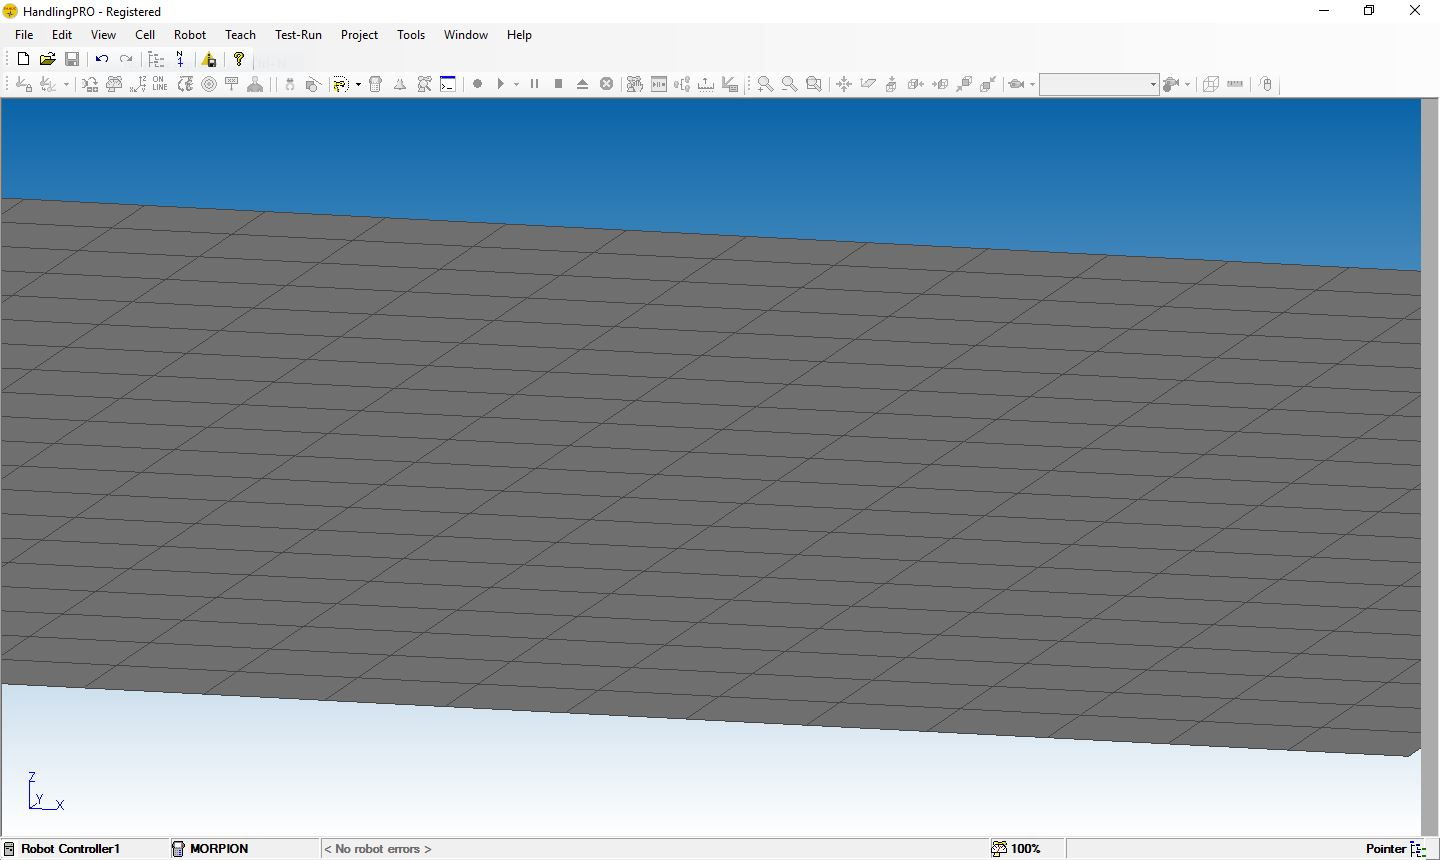
\includegraphics[width=8cm]{./roboguide.JPG}
			\caption{Interface du Roboguide}
			\label{fig:roboguide}
		\end{center}
	\end{figure}
	
	\pagebreak
	\mysubsection{2ème Semaine - 05/10 et 07/10}
	Dans cette semaine l'équipe a été divisé en deux groupes, et chacun a réalisé la même activité mais en jours différentes, le programmation du jeu de morpion (figures \ref{fig:morpion} et \ref{fig:morpion1}) et la planification des activités de la séquence 5. 
	
	\begin{figure}[H]
		\begin{center}	
			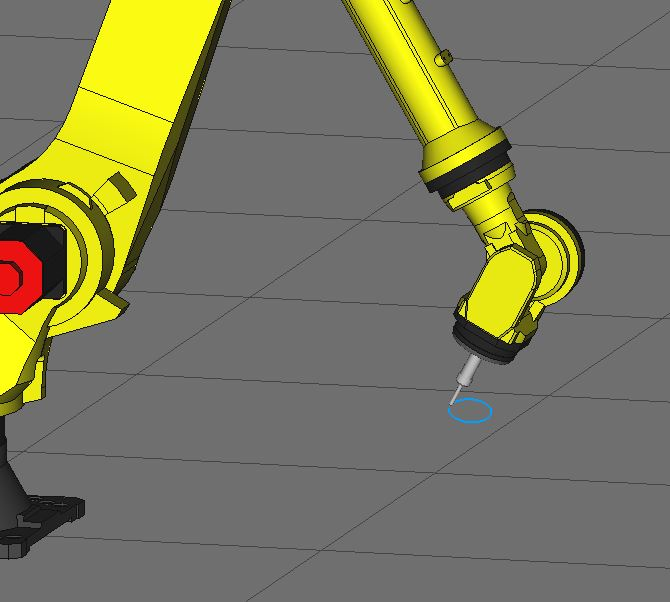
\includegraphics[width=8cm]{./morpion.JPG}
			\caption{Robot en faisant un circle}
			\label{fig:morpion}
		\end{center}
	\end{figure}
	
	
	\begin{figure}[H]
		\begin{center}	
			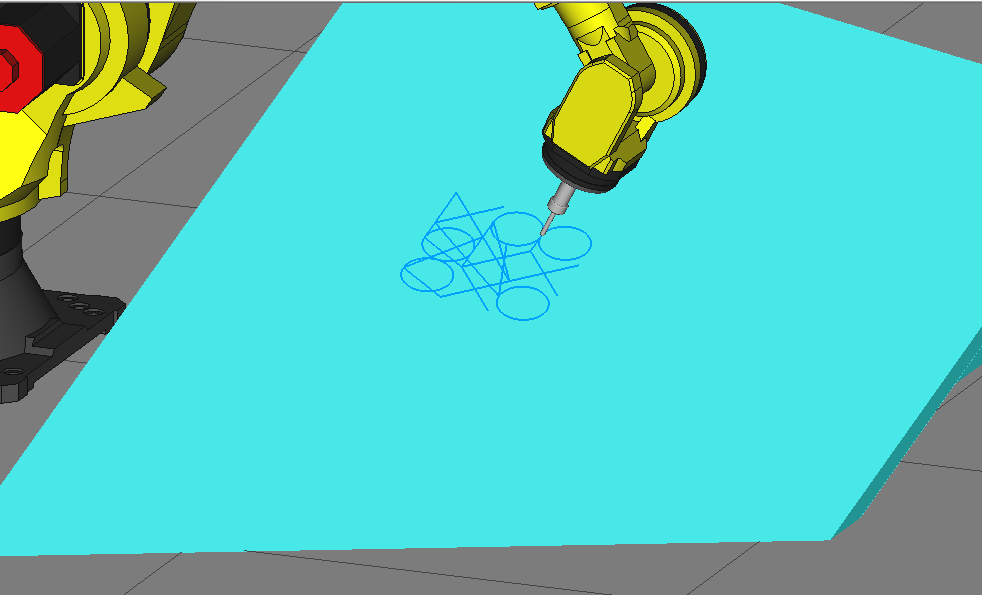
\includegraphics[width=8cm]{./morpion1.PNG}
			\caption{Partie du Jeu de Morpion, sur une table inclinée}
			\label{fig:morpion1}
		\end{center}
	\end{figure}
	
	\pagebreak
	\mysubsection{3ème Semaine - 12/10}
	L'activité réalisé dans cette semaine était la prise et dépose de boîte sur une table. Dans cette activité quelques choses ont été appris, comme la création d'un outil qui bouge (une pince pour exemple) et addition des éléments périphériques qui seront utilisés dans la simulation comme tables, boîtes et autres objets.
	
	
	\mysubsection{4ème Semaine - 19/10}
	Une réunion avec Mme Makarov a été realisé a propos  des progrès du projet et pour résoudre quelques doutes que n'ont pas été solutionné.  Après la réunion l'équipe a fait une petite auto-évaluation à propos de la bonne maîtrise du logiciel RoboGuide et début de l'étude de l’avant-projet des années dernières (compréhension de la consigne)
	
	\mysubsection{5ème Semaine - 26/10} 
	Pour trainer et étudier comment faire la simulation avec différentes objets, en binôme, programmes de simulation de prise et déposes des boîtes dans un four (figures \ref{fig:four}, \ref{fig:four1} et \ref{fig:four2}), pour différencier les deux simulations, chaque binôme a utilisé un type de pince différente. Et après quelques propositions de solutions pour l'avant-projet analysé la semaine antérieure ont été fait.
		
	\begin{figure}[H]
		\begin{center}	
			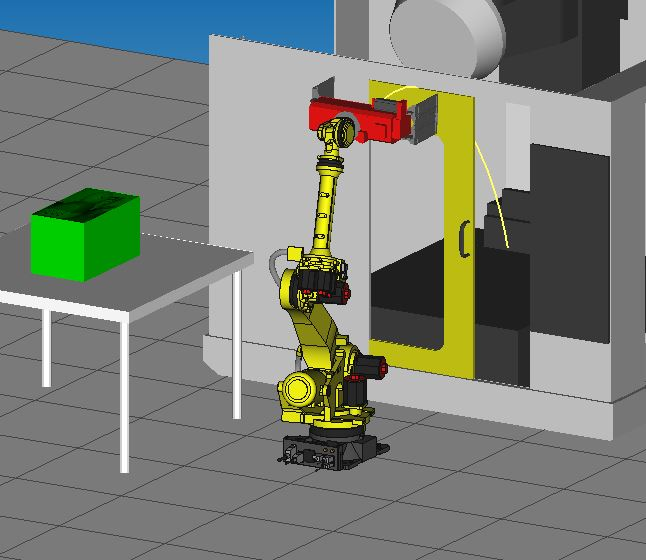
\includegraphics[width=8cm]{./four.JPG}
			\caption{Bras en train de bouger vers la boîte.}
			\label{fig:four}
		\end{center}
	\end{figure}
	
	\begin{figure}[H]
		\begin{center}	
			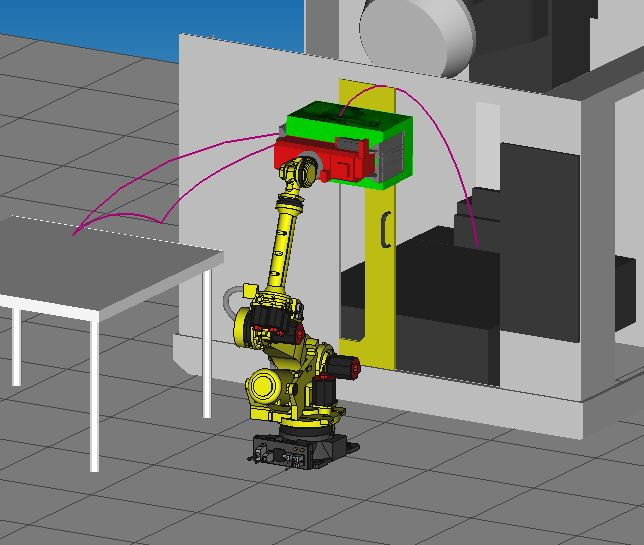
\includegraphics[width=8cm]{./four1.JPG}
			\caption{Bras en prennant la boîte.}
			\label{fig:four1}
		\end{center}
	\end{figure}
	
	\begin{figure}[H]
		\begin{center}	
			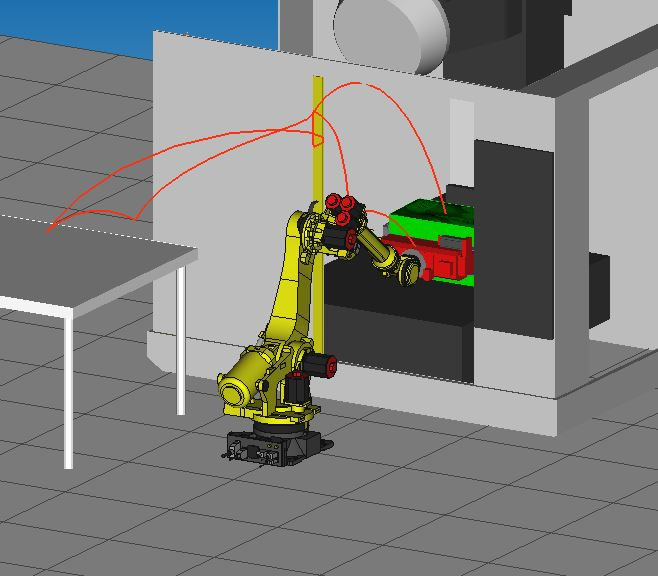
\includegraphics[width=8cm]{./four2.JPG}
			\caption{Bras en déposant la boîte dans le four.}
			\label{fig:four2}
		\end{center}
	\end{figure}
	
	\mysubsection{6ème Semaine - 02/11 et 04/11}
	Dans ces jours l'avant-projet de cette année a été lu et discuté, une séquence d'étapes a été proposé a fin de résoudre l'avant projet. Le sujet d'épreuve nº 1 a été pris en main et hypothèses ont été crée à propos de le même. Et l'équipe a discuté la organisation des étapes pour la préparation du rapport de la séquence.
		





\pagebreak \mysection{Discussion sur la méthodologie}


Avant de proposer n’importe quelle solution au problème en vue, c’est impératif de proposer une méthodologie de résolution plus générale, afin d’établir un savoir-faire autour du sujet et permettre le groupe d’atteindre une solution plus efficace et optimale.\\
Ce qu’on propose c’est un diagramme que lie le début du projet (le sujet) à la fin (une solution décrite par un document) à travers une série d’étapes bien définies. Le diagramme est présenté ci-dessous.\\


\begin{figure}[H]
	\begin{center}	
		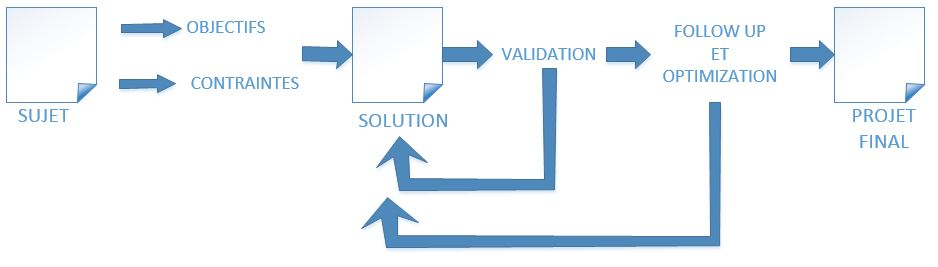
\includegraphics[width=15cm]{./diagrama.JPG}
		\caption{Méthodologie de projet}
		\label{fig:diagrama}
	\end{center}
\end{figure}



\vspace{20pt}
Le diagramme contient des objets (sujet, solution, projet final), éléments dérivés (objectifs, contraintes) et actions (valider, optimiser). On discutera brièvement toutes ses relations.
\begin{itemize}
	
\item Sujet : Document de spécification des besoins du client. Ordinairement ce document est composé par l’équipe avec le client, dans le cas des Olympiades il est déjà prêt.
\item 	Objectifs et contraintes : L’objectif est simplement ce que doit être atteint, décrit de manière simple et vérifiable. Les contraintes sont des limites que la solution doit respecter. Les deux sont dérivés du sujet, mais l’équipe doit ajouter contraintes supplémentaires afin de diminuer l’espace de solutions.
\item 	Solution : Ce que respecte les contraintes et accomplit les objectifs. Dans le cas des Olympiades une solution est composée d’une simulation dans le logiciel Roboguide.
\item 	Validation : Action d’évaluer une solution supposée afin de déterminer si, en fait, elle respecte les contraintes et accomplit les objectifs.
\item 	Optimisation : Action de critiquer la solution courant et proposer une autre solution que peut avoir une meilleure performance par rapport à une mesure de performance (temps total, coût, espace occupé, consommation d’énergie, etc.). 
\item 	Projet Final : Document que contient la description de la solution, la consolidation du projet et l’argumentation de la raison pour laquelle une entreprise quelconque devrait payer pour la solution proposée.
\end{itemize}

\vspace{20pt}
Cela dit, c’est facile de comprendre le flux du projet :
\begin{enumerate}
	\item On dérive les objectifs et les contraintes à partir du sujet.
\item	On propose des contraintes et hypothèses supplémentaires et on propose une solution. 
\item	On valide la solution, en mettant à l’épreuve les hypothèses faites dans l’étape dernière. Si la solution proposée n’accomplit pas les objectifs ou ne respecte pas les contraintes il faut retourner à l’étape 2 et vérifier quelle hypothèse était fausse ou quelle contrainte était excessive.
\item	Si la solution est validée, on a déjà une solution que marche. Dans cette étape il faut analyser la solution et proposer des améliorations, ou des solutions alternatives. Si on est satisfait avec la solution courant on passe à l’étape finale, autrement on retourne à l’étape 2 en proposant une autre solution.
\item	Dans cette étape il faut documenter la solution et la présenter en détail, avec des images et des chiffres, dans un document appelé projet final.

\end{enumerate}

\mysection{Analyse du énoncé d'année précédente}

\mysubsection{Choix des robots}
Il existe deux emplois différents à faire par des robots : la palettisation et le remplissage des caisses avec des bouteilles.\\
  
Dans les spécifications du projet, pour la palettisation est prévue que le préhenseur en charge aurait le poids de 25.8 kg et le robot choisi doit supporter cette charge. De plus, le bras du robot devra atteindre la zone des caisses et de palettes, ainsi il devra avoir un rayon d’action minimum égal le milieu du segment que relie les deux zones et aussi  le milieu du segment de la hauteur des caisses sur le convayeur et la zone des caisses , équivalent à 2075mm.La figure dessous représente ce calcul: \\

\begin{figure}[H]
	\begin{center}	
		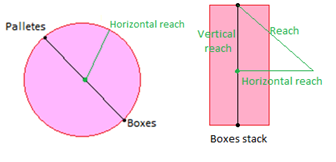
\includegraphics[width=8cm]{./Karol/Calculo.png}
		\caption{Répresentation du calcul de rayon d'action}
		\label{fig:representation}
	\end{center}
\end{figure}

Pour le remplissage des caisses avec des bouteilles est prévu que le préhenseur en charge aurait le poids de 5.47 kg et le bras du robot devra atteindre la zone des convoyeurs de bouteilles et des caisses, de la même façon que le robot antérieur, ce robot devra avoir un rayon d’action minimum égal le milieu du segment de relie les deux zones, équivalente a 414mm. 

\pagebreak
Alors, à partir de ces spécifications et considérant les meilleurs coûts-bénéfices en termes de production ont été choisis les robots suivants : \\




\underline{Robot de palettisation: robot controller 1}\\

\begin{figure}[H]
	\begin{center}	
		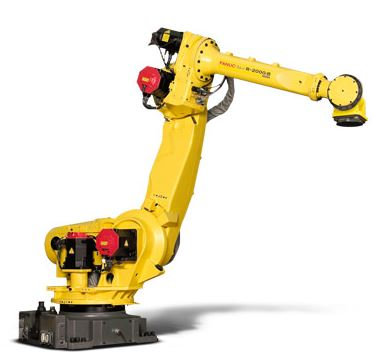
\includegraphics[width=8cm]{./Karol/figura1.JPG}
		\caption{Modèle: R-2000iB/100H-2}
		\label{fig:R-2000iB/100H-2}
	\end{center}
\end{figure}

\begin{itemize}
	\item Capacité de charge maxime admissible au poignet : 100 kg
	\item Rayon: 2655mm
	\item Axes: 5
\end{itemize}
\vspace{10pt}

Les autres robots de la série R-2000iB ont plus grande capacité de charge et rayon d’action, ainsi ils ont aussi plus grands coûts. Pourtant, parmi les robots de palettisation de cette série que répond aux spécifications du projet, c’est le robot avec le plus grand coût-bénéfice. \\

\underline{Robot de remplissage des caisses avec des bouteilles: robot controller 2 and 3 }\\


\begin{figure}[H]
	\begin{center}	
		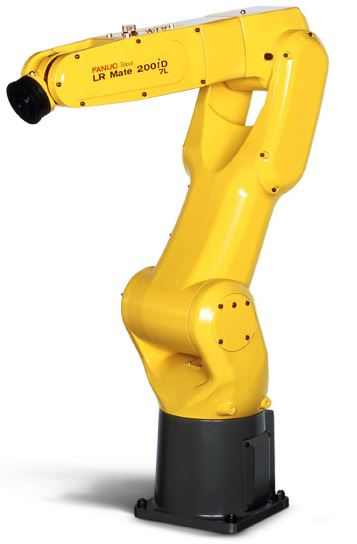
\includegraphics[width=4cm]{./Karol/figura2.JPG}
		\caption{Modèle: LR Mate 200iD/7L}
		\label{fig:LR_Mate_200iD/7L}
	\end{center}
\end{figure}
\newpage
\begin{itemize}
	\item Capacité de charge: 7 kg;
	\item Rayon: 911mm
	\item Axes: 6
	\item Bras long
\end{itemize}

\vspace{20pt}
Pour cette finalité, tout le robot poli articulé marche, mais la série LR Mate est spécifique pour robots plus petits et légers. Ainsi, c’est plus approprie pour les bouteilles. Un autre robot de cette série LR Mate 200iD/7LC a les mêmes spécifications techniques du robot choisi, mais il est de la line \textit{cleam room} robot, que il n’est pas nécessaire dans ce projet. Ainsi, pour répondre aux spécifications du projet le choix du robot LR Mate 2 – iD/7L est justifiée. \\
On a besoin de définir la quantité de robots. Pour remplissage des caisses avec des bouteilles, on a quatre bouteilles en 1.5s (sur chaque convoyeur). En considérant que le convoyeur doit être arrêté dans le moment que le robot prise les bouteilles, on doit ajouter le temps de prise. Ainsi, huit bouteilles prennent 1.75s. À partir de la simulation, en considérant la vitesse nominale, on trouve que le cycle complet du robot (20 bouteilles par caisse) prends 12.5s, c’est équivalent à 2.5s par quatre bouteilles. Avec ça, on peut conclure qu’on a besoin de deux robots pour le remplissage des caisses avec des bouteilles, parce qu’un unique robot ne serais pas suffisant pour répondre aux cadences des bouteilles et plus qu’un laissera le robot inoccupé pour une grande période. \\
On sait que deux caisses sont remplies avec des bouteilles en 12.5s. De plus, on peut ajouter 2s relatif au pas de deux caisses. Pourtant, le flux est des deux caisses en 14.5s, c’est équivalent à 7.25s pour chaque caisse. En considérant le temps technologique de prise et dépose, la palettisation prend le temps de 5.55s. C’est un temps possible pour le robot, ainsi on peut choisir seulement un robot de palettisation. 
 


\mysubsection{Positionnement des robots}
Une fois que les robots ont été déjà choisi, la deuxième étape consiste à déterminer le positionnement des robots par rapport aux fournitures, dont positions ont été déjà fourni dans la consigne de l’avant projet (ou dans un cas réel, cela représente le vrai positionnement des fournitures ou des machines dans l’usine).\\

Premièrement, comme les convoyeurs des caisses ont une hauteur de 1085 mm et le rayon de travail des robots qui vont remplir les caisses est 911 mm, on a besoin d’utiliser un piédestal pour eux. On sait bien qu’utiliser un piédestal ajoute des frais au projet, et à mesure que la hauteur du piédestal augmente, son prix augmente aussi. Donc on doit choisir le piédestal le plus bas qui permet au robot de bien réaliser ses activités, afin de réduire les frais. Ce choix implique une analyse de toutes les tailles de piédestal disponible dans le marché et leur prix, qu’on n’a pas trouvé, et il y a une relation aussi avec la distance horizontale entre le robot et le convoyeur. Empiriquement, on doit choisir un piédestal un peu plus bas que le convoyeur (environ 1000 mm de hauteur). La distance horizontale par rapport au point le plus loin qu’il doit placer une bouteille doit être inférieure, au moins de 50 mm, au rayon de travail du robot (861 mm). Dans la solution de l’avant-projet, ils ont choisi une hauteur de 1100 mm et une distance horizontale d’environ 775 mm. 

Pour le robot de palettisation, une fois qu’on doit palettiser 9 couches de caisses sur une palette qui est sur un convoyeur totalisant 3023.5 mm de hauteur et le rayon de travail du robot est de 2655 mm, on a besoin aussi d’un piédestal. En considérant que les caisses doivent être empilés pour la haute et que la distance entre les caisses remplies dans le convoyeur et la position la plus loin dans la palette est d’environ 1200 mm, le piédestal doit avoir au minimum 1000 mm. Ils ont choisi une hauteur de 1400 mm, et le robot est placé d’une façon équidistant entre le convoyeur de caisses et le point le plus loin de la palette qui est remplie. 

Peut-être s’ils avaient choisi des piédestal plus bas pour les trois robots, ils seraient arrivés dans uns solution moins chère et qui marche aussi bien. Pour avoir une solution optimale dans ce cas-là, on a besoin de simuler le programme en augmentant les hauteurs des piédestal. Mais pour le positionnement horizontale des robots, nous sommes complètement d’accord avec ce qui a été fait.

\mysubsection{Mouvement des robots}
Pour finir tous les éléments de la simulation, on doit ajouter aussi la laveuse / sécheuse, les grillages de sécurité et un contrôleur pour les trois robots. Placer le contrôleur dehors de la zone de sécurité facilite beaucoup le fonctionnement de la cellule pour éviter que les personnes rentrent dans la zone de sécurité. L’image \ref{fig:rap3} montre la cellule robotique.

\begin{figure}[H]
	\begin{center}	
		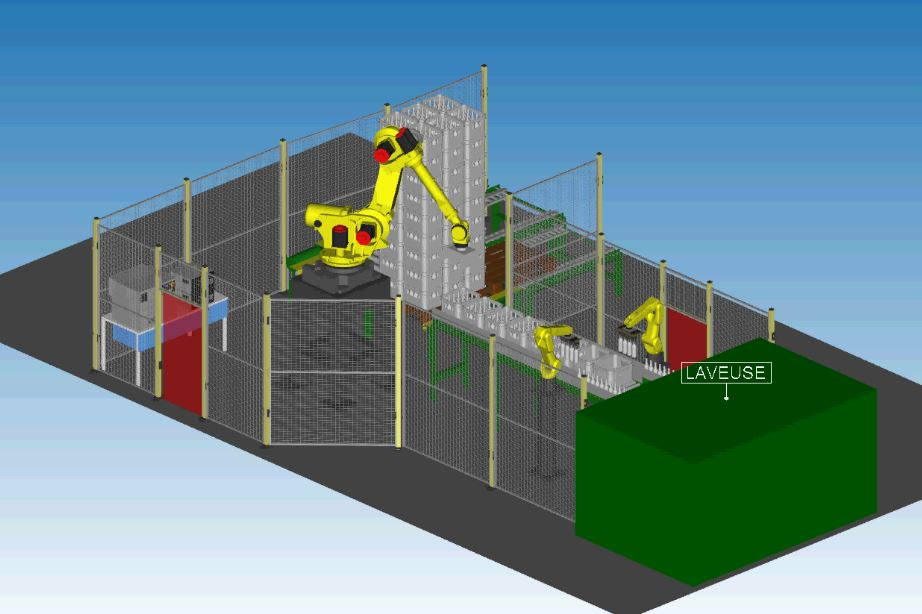
\includegraphics[width=8cm]{./rap3.JPG}
		\caption{La cellule robotique.}
		\label{fig:rap3}
	\end{center}
\end{figure}

Ensuite, on doit choisir les trajectoires des robots. Pour les robots des caisses, on doit se rassurer que les bouteilles sont mises par la haute et qu’elles ne vont pas frapper d’autres objets. Pour cela, on rajoute un point CNT100 au début du convoyeur et un point CNT10 sur la position voulue pour les bouteilles, dans une hauteur de 600 mm (caisse + bouteille) par rapport au convoyeur, et un point FINE dans la position voulue (cette position et la dernière position de rapproche vont changer avec un offset pour correctement remplir la caisse de cinq lignes de quatre bouteilles). On peut utiliser les mouvements JOINT pour les robots, qui sont plus rapides et suffisant dans ce cas. Les trajectoires sont illustrées dans la figure \ref{fig:rap1}. C’est convenable d’aligner les robots, la caisse et les quatre bouteilles avant de les prendre, en arrêtant le convoyeur de caisses dans cette position.

\begin{figure}[H]
	\begin{center}	
		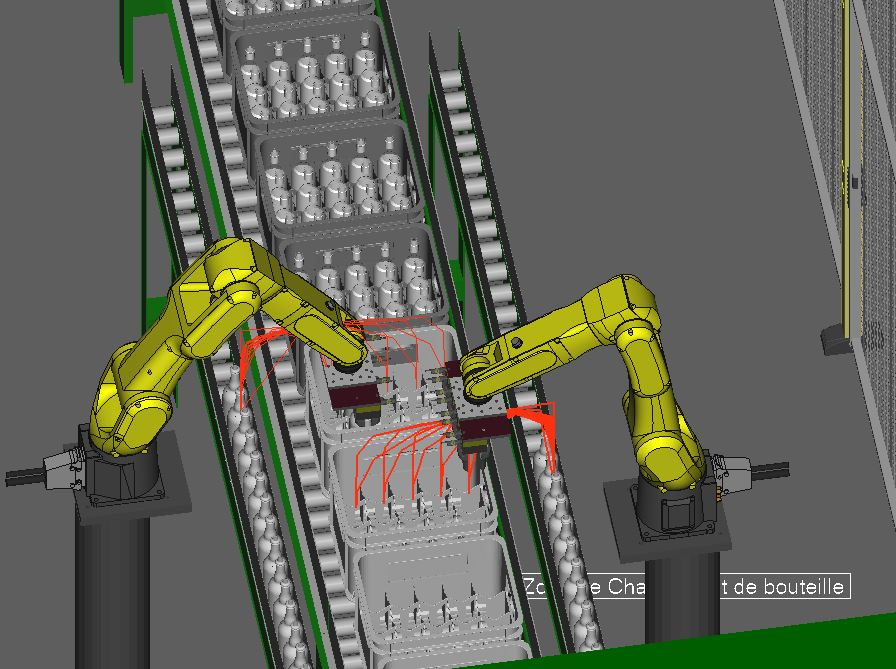
\includegraphics[width=8cm]{./rap1.JPG}
		\caption{Procès de remplissage des caisses.}
		\label{fig:rap1}
	\end{center}
\end{figure}

On peut utiliser la même idée pour générer le mouvement du robot de palettisation, sauf que pour lui, on va avoir besoin d’utiliser l’offset dans tous les axes (X, Y et Z) pour les trois points (les deux points de rapproche et le point de dépose). Ce robot doit empilé deux caisses dans les palettes avant que les autres finissent de les remplir pour que le convoyeur puisse bien marcher. La figure \ref{fig:rap2} illustre la trajectoire de ce robot.

\begin{figure}[H]
	\begin{center}	
		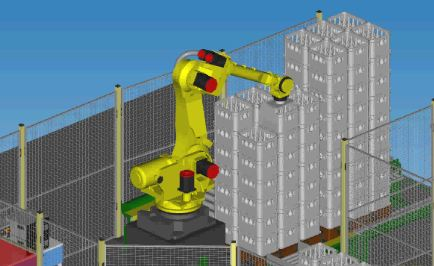
\includegraphics[width=8cm]{./rap2.JPG}
		\caption{Procès de palettisation.}
		\label{fig:rap2}
	\end{center}
\end{figure}

Pour finir, on peut ajouter des éléments DCS dans cette cellule, qui ne sont pas vraiment nécessaires dans ce cas, mais c’est toujours bien de les mettre dans une cellule robotique. Comme la probabilité d’avoir une personne dans la zone de sécurité est faible, on peut simplement éteindre les robots lorsqu’il y a une personne dans cette zone (probablement pour la maintenance des robots et des machines).







\pagebreak
\mysection{Difficultés trouvées}
Dans la deuxième étape de la méthodologie proposée, on devait formuler des hypothèses pour permettre la résolution du problème. Une telle hypothèse était la séparabilité entre les deux différentes tâches (remplissage et palletisation), c'est à dire, trouver une solution spécifique pour chaque processus et les ajouter, est une solution global. Cette hypothèse a été considéré si on rassure que le cadence de production soit la même pour les deux processus.



  
\mysection{Conclusion}
Comme on peut voir dans ce rapport, l'équipe a ressui obtenir les notions basique nécessaires pour participer aux olympiade soit en gestion de projet, soit en niveau technique, en apprenant comment utiliser le logiciel. 

%\todo{
%Introdução+objetivos
%1 parte: contando o que fizemos na sequencia 5
%
%2 parte: análise do enunciado do ano anterior
%
%
%
%
%Atividades Realizadas
%
%Colocar o que fizemos em cada semana (em um texto único). 
%Análise do enunciado do ano anterior
%Escolha do robo;
%1)	Enunciado: resumo do enunciado e ver o que precisa ser seguido a risca, analisar o diagrama ASM;
%
%2)	Venda: com engenharia reversa. Ex. Problema numero 1: escolha do robo; problema 2: movimentação e posicionamento do robo; problema 3: elementos de simulação 
%
%Critica
%
%Análise do ASM e reler e ridigir o enunciando enunciando as variaveis livres do ano anterior
%
%Durante esta sequencia, os 
%
%
%}






























\bibliographystyle{plain}
%\bibliography{bibliografia}
\end{document}